\documentclass[11pt,twoside,a4paper]{article}
\usepackage{graphicx}
\usepackage{amsmath}
\usepackage{mathrsfs}
\usepackage{graphicx}
\usepackage{float}
\usepackage[parfill]{parskip}

\begin{document}
\setcounter{secnumdepth}{0}
\title{M4R}
\date{March 2nd, 2019}
\author{Anthony Webster CID 01051827}
\maketitle
\section{Introduction}
We seek to create an efficient solver of the steady Navier stokes equations in an arbitrary domain in $H_{div}$ space. The steady Navier Stokes equation are as follows : 
\begin{align}
u \cdot \nabla u &= -\nabla p + \mu \nabla^2 u + F \\
\nabla \cdot u &= 0
\end{align}
Not that from working in the $H_{div}$ space the second equation is naturally satisfied globally.
\\
First we will describe the classic Finite Element Method, its advantages and disadvantages, hence explaining why we are using a modified method. Secondly we will explain a number of definitions and tools used in the project and which may be unfamiliar to some readers. Then we will show how to find the weak form of the equations and build different parts of our solvers. Lastly we will consider some example cases and deduce that the algorithm converges to the right result at satisfactory rates.\\


\section{Classic Finite Elements Method}
The finite element method (FEM) is a numerical method which approximates the solution to an exact partial differential equation [5]. The property that it works on arbitrary domains, as opposed to the finite difference method which finds the exact solution to an approximated discretized partial differential equation, is one of the reasons it is widely used in research, industry and this project.\\
\\
We will now consider the case of applying the FEM to the stokes equations using the more classic lagrange finite element.\\
\begin{align}
0 &= -\nabla p + \mu \nabla^2 u + F \\
\nabla \cdot u &= 0
\end{align}
As seen in Common and Unusual Finite Elements [7], the lagrange finite element approximates a function on a cell using polynomials of degree $q$ defined by their pointwise values at an array of points (such as a uniform lattice).\\
For instance let us approximate $f = sin(x)$ from $0$ to $2 \pi$ using 1D first order lagrange finite elements. We approximate the function on each of the four cells by a linear function. This linear function is defined on each cell using two points in it, the two edge points. Hence we get figure 1, where the blue curve indicates our approximation and the red one the exact function. In practice one can consider $f$ to be the sum of these linear functions. Note that this element is continuous across the "edges" of a cell, since regardless of cell the value of the interpolated function at the "edge" will be identical. This concept can be extended to 2D.\\
\begin{figure}
  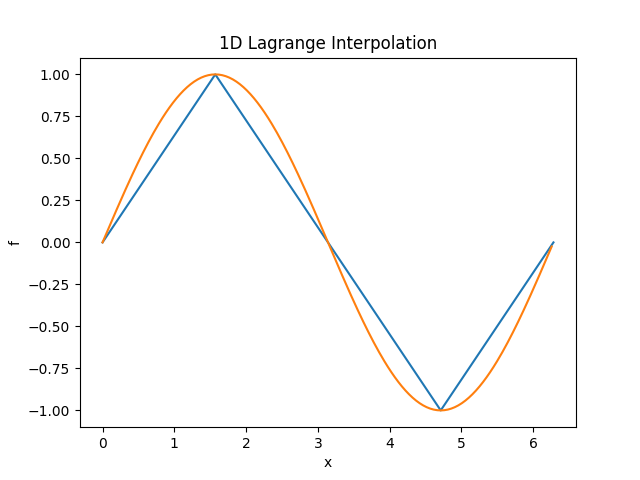
\includegraphics[width=\linewidth]{ex_1D_LG.png}
  \caption{4 element First Order Interpolation Example}
\end{figure}
\\
It follows that we first cut up our domain into a mesh. Commonly these meshes are made up of triangles for simplicity, although squares or even curved elements for simulations on a sphere are also used. Then we approximate $u$ and $p$ using the lagrange element. Hence we get that for instance $u$ is the sum of a set of known piecewise linear functions (as they are determined by the mesh) but with unknown coefficients. The aim of the rest of the method is to determine these unknown coefficients.\\
For that end we need to find what is called the weak form of the equation. We multiply (3) by an arbitrary function $v$. Hence we get :
\begin{align*}
\int_{\omega} -v \cdot \nabla p + \mu v \cdot \nabla^2 u dx = -\int_{\omega} v \cdot F dx
\end{align*}
Since our domain $\omega$ is cut out into triangles we can cut the integral into triangles and work on each one individually. Hence for each cell $e$ in $\omega$ we get : 
\begin{align*}
\int_{e} p \nabla \cdot v + \mu v \cdot \nabla^2 u dx =  -\int_{e} v \cdot F dx
\end{align*}
However since $u$ and $v$ will be approximated by functions which may be discontinuous in their derivatives $\nabla^2$ may not be defined. Hence we need to use integration by parts to get :  
\begin{align*}
\int_{e} p \nabla \cdot v - \mu \nabla v \cdot \nabla u dx = -\int_{e} v \cdot F dx
\end{align*}
Finally multiplying (4) by a similar pressure test function $q$ and adding it to the left hand side of the above we get :
\begin{align}
\int_{e} p \nabla \cdot v - \mu \nabla v \cdot \nabla u dx + \int_{e} q \nabla \cdot u dx = -\int_{e} v \cdot F dx
\end{align}
Now we use the fact that $q$, $v$, $F$, $u$ and $p$ are a sum of known linear functions and coefficients.\\
Pulling out and removing the coefficients of $v$ we get that :
\begin{align*}
 \int_{e} \sum_i \sum_j (  p_j \phi_j \nabla  \cdot \Phi_i - \mu \nabla \Phi_i \cdot u_j \nabla \Phi_j +   \phi_i u_j \nabla \Phi_j) dx = -\int_{e} \sum_i \phi_i F_i \phi_i dx
\end{align*}
Combining all the triangles we can eventually turn our problem into a matrix equation of the form :
\begin{align}
M x = b
\end{align}
Where x is a vector of coefficients of $u$ and $p$.\\
We can solve this using a variety of linear systems solvers. Note in particular that since the majority of basis functions $\Phi$ and $\phi$ are $0$ in any given triangle the matrix $M$ will be sparse.\\
While we locally enforced the divergence-free equation by including it in the weak form, the global flow may not be divergence-free. In order to achieve that more complex mathematical tools would be required.\\
Now apply this to the manufactured solution :
\begin{align*}
u_x &=  sin(2 \pi y) cos(2 \pi y)  sin(2 \pi x)^2 \\
u_y &= -sin(2 \pi x) cos(2 \pi x)  sin(2 \pi y)^2 \\
p &= sin(2 \pi x)^2 sin(2 \pi y)^2 \\
F &= \nabla p - \mu \nabla^2 u
\end{align*}
Where $F$ was selected specifically to ensure that any given $u$ and $p$ are solutions.
Using the above and implementing it in firedrake we get figures .On a mesh with vertices we get an error of about.

\section{Tools and Definitions}
\subsection{Brezzi-Douglas-Marini Element}
The paper Common and Unusual Finite Elements [7] states that the BDM space on one triangle $K$ is composed by polynomials of order $q$ defined by the normal component on each edge. If $q > 1$ it is also defined using the integration against gradients of the polynomials on the triangle. If $q > 2$ we then also use the integration  against curls of $b_K P_{q-2}(K)$ where $b_{q-2}$ is the  cubic bubble function associated with $K$ and $P_{q}(K)$ is the set of polynomials defined on $K$.\\
This finite element, combined with the DG element for pressure, discretizes the function space H(div). A property we thus get from simply working in BDM is that our solution will be exactly divergence free globally and locally.
Additionally we will be able to employ an enhanced lagrangian preconditioner thanks to the global divergence free property [2].\\

However unlike the lagrange elements we can no longer set a dirichelet boundary condition's tangential component. Therefore we need to find alternative approaches to enforce these conditions.
Additionally some operations (such as the curl) are undefined in this space. Due to possible discontinuities at the boundaries we also have to be carefull with all boundary integrals.\\

In general the weak form will be far more involved.


\subsection{Discontinous Galerkin and BDM-DG Mixed Space}
The discontinous Galerkin Element space is the space of piecewise linear continuous functions.\\
Combined with the BDM space we obtain a mixed finite element space which approximates the $H_{div}$ finite element space.\\

\subsection{Newton's Method}

Newton's method is a generalized method for solving non-linear matrix equations of the form :
$$
F(x,y) = 0
$$
Where $F$ is a vector function and $x$ is vector of unknowns. Note that $F$ may be non-linear and have constant components.
For instance we could have $ F = x^T A x + M x - b$, where A and M are constant matrices and b is a constant vector.\\ 
We start with a guess $x = x_0$ and then determine the Jacobian of $F(x)$, call it $DF(x)$.\\
We determine the jacobian by calculating the Gateaux derivative, defined as follows [12] :
\begin{align}
DF_{x_n}(\Delta x) = lim_{t \rightarrow 0^+} \frac{F(x_n+ \epsilon \Delta x) - F(x_n)}{\epsilon}
\end{align}
We then use the vector taylor expansion :
\begin{align*}
F(x_{n+1}) = F(x_n) + DF_{x_n}(\Delta x) \Delta x 
\end{align*}
Hence we get the algorithm :
\begin{align}
DF_{x_n}(\Delta x) \Delta x = - F(x_n)\\
x_{n+1} = x_n + \Delta x 
\end{align}
We solve for $\Delta x$ using $x_n$ and the taylor expansion approximation and then use this result to determine $x_{n+1}$.
This is a linear problem which can be solved via an Lu Factorization for instance.\\
Note that the Newton's method only converges and is unique if it is within a ball around the solution [10-11].

\subsection{Preconditioners}

We will first describe how preconditioners, such as the Schur Preconditioner work in general. We see this in the book Multilevel Block Factorization Preconditioners [4] on pages 49 to 51.\\
Take the system :\\
$$
Mx = b
$$
Where $M$ is a very large matrix, assumed for simplicity to be symmetric, $x$ and unknown vector we need to solve for (in our case this will be a vector of coefficients for both $u$ and $p$) and $b$ a constant vector. If $M$ is a symmetric positive definite sparse matrix then $M$ applied to a vector is cheap to compute. Hence we can easily find $r$ the residual such that :\\
$$
r = b - Mx
$$
We then use the resulting $r$ in order to provide a correction on our result.\\
However $M$ may not be well-behaved. In fact in our problem we know it is usually not.\\
In this case we use a preconditioning matrix, $P$ to map the system in such a way that $P^{-1}$ is cheap to compute, this operation can easily be parallelized and the condition number, the ratio of largest and smallest eigenvalue which describes the behaviour of the system [13], is lowered.
We then numerically solve the transformed and hopefully better behaved system : 
$$
P^{-1}(Mx-b) = 0
$$ 

\subsection{Notation}

Let $\{ a \} = a_+ + a_-$. \\
This is an average term. Due to discontinuities of our space on facette elements integrals over facets from integration by parts on an individual element will not dissappear necessarily, hence these terms remain. Additionally, since we cannot use dirichelet boundary conditions, weak penalty terms will also use this operation.\\
When the mesh is setup the program ensures each facette of each cell has a positive and negative side. Whenever we call this term on a facette integral it thus follows the formula above, where $a_+$ is the value of $a$ on the positive side $a_-$ on the negative side.\\
For integrals over outer facettes we explicitly write out the formula for clarity.\\
\\
Similarly let $J(a) = a_+ - a_-$\\
This is a jump term. Note that this operation is $0$ in continuous space, which is where we assume the physical fluid velocity and pressure to be.\\
\\
We may have surface integrals over interior facettes and exterior facettes, which are on the computational boundaries.\\
In the first case the integral of $a$ is $\int_\Gamma a dS$ while in the latter we note $\int_{\delta \Omega} a ds$.\\
This is used both for additional clarity and because it is the notation in the code.


\section{Implementing the $H_{div}$ Solver}
Since we have two problem terms we will deal with each separately. Hence we will first consider the stokes equation, ignoring the advection term and focusing on the viscosity term for now :
\begin{align}
0 &= -\nabla p + \mu \nabla^2 u + F  \\
\nabla \cdot u &= 0
\end{align}

\subsection{Stokes Equation}
We start off by cutting our computational domain $\Omega$ into a set of cells $e$. As discussed above it is now required to find the weak form of equations (9) and (10).
For this purpose let us introduce two test functions, $w$ in BDM for velocity and $q$ in DG for pressure.
Let us multiply equation (9) by $v$ and integrate over the domain as seen in the first section.
\begin{align*}
\int_\Omega v \cdot F dx &= \int_\Omega (v \cdot \nabla p) dx - \int_\Omega (\mu v \cdot \nabla^2 u) dx
\end{align*}

Again we can work on each cell $e$ individually and them sum it all up, hence get :
\begin{align*}
\sum_e \int_e v \cdot F dx &= \sum_e (\int_e (v \cdot \nabla p) dx - \int_e (\mu v \cdot \nabla^2 u) dx)
\end{align*}
Focusing on the viscosity, or second, term we get via integration by parts :
\begin{align*}
\int_e (v \cdot \nabla^2 u) dx = - \int_e \nabla_h(v) : \nabla_h(u) dx + \int_\Gamma 2 \{ v_i n_j \} \{ \frac{\partial u_i}{\partial x_j}\} dS
\end{align*}
The first term can be summed up to an integral over $\Omega$ and the second one is asymmetrical. We can add a term to make it symetrical. This helps with numerical stability of the final matrix equation. Additionally some linear solvers take advantage of this structure.\\
Hence this term becomes :
\begin{align*}
-  \int_\Omega \nabla_h(v) : \nabla_h(u) dx + \sum_e( \int_\Gamma 2 \{ v_i n_j \} \{ \frac{\partial u_i}{\partial x_j}\} dS + \int_\Gamma 2 \{ u_i n_j \} \{ \frac{\partial v_i}{\partial x_j}\} dS)
\end{align*}
$u$ should be continous in the physical space thus the added term will cancel out. Hence this does not change the equation.\\
\\
Now we also add the term $\alpha \int_\Gamma \frac{1}{h}  J(v_i) J(u_i) dS$. According to sources [3] provided that  $\alpha$ is larger than $10$ numerical stability is increased.\\
$J$ is the jump notation.\\
The numerical value of $h$ is the average distance of a side. In our case we defined it as the average cell-volume over the length of the facettes between them for each individual facette element $\Gamma$.\\
The $J(u_i)$ term makes this integral $0$ in continous space so this does not change the solution.\\
\\
As mentioned in the BDM definition section we cannot set the tangential component of a dirichelet boundary condition in the conventional finite element manner.  So instead we use penalty terms, which should be $0$. This pushes the solution towards respecting the boundary conditions. In practice this just means taking all the terms over the edge of a cell and considering them on the edge of the domain instead.\\
 Hence our final viscous term becomes :\\
\begin{align*}
&-  \int_\Omega \nabla_h(v) : \nabla_h(u) dx + \sum_e ( \int_\Gamma 2 \{ v_i n_j \} \{ \frac{\partial u_i}{\partial x_j}\} dS + \int_\Gamma 2 \{ u_i n_j \} \{ \frac{\partial v_i}{\partial x_j}\} dS \\
&- \alpha \int_\Gamma \frac{1}{h}  J(v_i) J(u_i) dS \ ) + \int_{\partial  \Omega} v_i n_j \frac{\partial(u_i + u^0_i)}{\partial x_j} + (u_i + u^0_i) n_j\frac{\partial v_i}{\partial x_j} ds - \alpha \int_{\partial \Omega} \frac{1}{h} v_i(u_i-u^0_i)ds
\end{align*}
Where $u^0_i$ are the boundary values.
We will call this term $\eta_\mu$.\\
Back to our original equation we get : 
\begin{align}
\int_\Omega v \cdot F dx &= \int_\Omega v \cdot \nabla p dx - \eta_\mu
\end{align}
Let us consider the continuity equation again :
\begin{align*}
\nabla \cdot u = 0
\end{align*}
Multiplying by $q$ and integrating we get :
\begin{align*}
\int_\Omega q \nabla \cdot u dx = 0
\end{align*}
This is $0$, so we substract this from the weak formulation $(3)$ we obtained, getting one weak formulation which includes both pressure and velocity while also keeping symmetry. \\
We need this since we want to turn the entire system into a single matrix equation which includes all the conditions.\\
Integrating by parts the pressure term and using the divergence theorem get :
\begin{align}
\int_\Omega v \cdot F dx &= \int_\Omega \nabla \cdot (p v) dx - \int_\Omega  p ( \nabla \cdot v) dx - \int_\Omega q (\nabla \cdot u) dx  - \eta_\mu
\end{align}

\subsection{Applying the Schur Preconditioner to our problem}
In an effort to get our iteration count to be independent of mesh-size, we will apply a Schur preconditioner similarly described in chapter 3 of Multilevel Block Factorization Preconditioners [4] as well as in source [2].\\
This is a well-known method, however as we will be modifying it, we will quickly describe it as well.
Our sytem effectively amounts to solving a matrix equation of the form :
$$ 
\begin{bmatrix} 
A         & B^{T}\\
B         & 0 \\
\end{bmatrix}
\begin{bmatrix} 
u    \\
p     \\  
\end{bmatrix}
=
\begin{bmatrix} 
b    \\
0     \\  
\end{bmatrix}
$$
Where $B$ is the discretized divergence operator and $B^T$ the discrete gradient operator. $A$ contains the viscous term.
Setting $S = - B A^{-1} B^{T}$, we can factorize the above and get an expression whose inverse is : 
$$
\begin{bmatrix} 
I         & - A^{-1} B^{T}\\
0         & I \\
\end{bmatrix}
\begin{bmatrix} 
A^{-1}   & 0\\
0       & S^{-1} \\
\end{bmatrix}
\begin{bmatrix} 
I & 0\\
 - B A^{-1}       & I \\
\end{bmatrix}
$$
Hence, if we can find $A^{-1}$ and $S^{-1}$ we can easily solve the equation. We solve both via a Lu factorization.\\
We solve for $A^{-1}$, or to be exact the operation $A^{-1}v$ via an Lu Factorization. The Lu factorization is a direct solver, and thus is innefficient. The algorithm would have to be performed in a sequential manner, preventing usage of parallelisation. We did mitigate this through the usage of the "mumps" sub-routine. Additionally there was an  However more efficient implementations would require this to be modified.\\
 However $S^{-1}$, the inverse of the shur complement is difficult to determine because it is usually dense. However research has shown [2 \& 9] that we can solve this issue by using a "grad-div" stabilization method. We add the term $\gamma \nabla \cdot v \: \nabla \cdot w$ to the equation (!). Note that this term is 0 in continuous space. We thus get : 
\begin{align}
\int_\Omega w \cdot F dx &= \int_\Omega \nabla \cdot (p v) dx - \int_\Omega ( p \nabla \cdot (v)) dx - \int_\Omega q (\nabla \cdot u) dx  - \eta_\mu + \int_\Omega \gamma \nabla \cdot u \: \nabla \cdot v dx
\end{align}
This doesn't change the equation, thus should result in the same solution. However acoording to the same papers [2 \& 9] we can then approximate $S$ by the pressure mass matrix. We then perform ILu in order to solve for $S^{-1}$. ILu performs the Lu Factorization on various blocks of the matrix, allowing it to be parallelised.

\section{The Continuation Method}
Now we include a modified advection term : 
\begin{align}
0 = RHS - LHS - c ( u \cdot \nabla u) 
\end{align}
Where LHS and RHS are the Left hand and Right hand side of equation (5). Note that this is equation is not linear, hence we will need to use Newton's method.\\ 
Given the navier stokes equations we could try to naively set $c = 1$ and then use Newton's method applying the above preconditioning and discretization methods. However at high Reynolds number this approach quickly fails unless the mesh is refined, leading to high computational cost.\\
Hence, in such cases, we will initially set $c$, referred to as the advection switch, to $0$. Applying the solver to $c = 0$ we should easily find a solution. Using this solution as a starting point we then calculate the derivative of (6) with respect to the advection switch.\\
We then solve again with the non-linear solver using the previously obtained solution for $c = 1$. If this fails we reduce $c$ until it works. We then repeat this procedure until $c = 1$.\\
 This allows us to rapidly solve simple problems, for which the advection switch is unecessary, as well as more complex problems, since we can use more efficient step-size in $c$ initially saving iterations, automatically.\\
In some circumstances however even with a variable step-size in $c$ we fail to obtain a solution. In our code if the step-size is below $10^{-3}$ our solver stops and fails.

\subsection{Navier Stokes Weak Form}
TODO
\section{Stability Analysis}

While we are mainly interested in the steady-state solution of the navier-stokes equation we also need to consider whether or not the solution is stable. To that end we need to solve a full navier stokes, including the time derivative. This will be used to determine if small perturbations of the solution die down.
\subsection{Time stepping method}
In practice our problem amounts to the following, very generalized, equation : 
\begin{align}
F(u) = 0
\end{align}
Where F is some function. this is in practice how the firedrake non-linear solver solves the equation.\\
If we add in the time-terms we get :
\begin{align}
\frac{\partial u}{\partial t} + F(u,p) = 0
\end{align}
While we could try and solve this equation directly using Backwards Euler or Midpoint Rule testing shows that this does not converge. Instead we use Picards iteration along with the Midpoint rule as described in the following equation :
\begin{align}
u^{n+1} - u^n + \Delta t (\frac{1}{2}G(u^n,p^n) + \frac{1}{2} G(u^{n+1},p^{n+1}) + ( u^n \cdot \nabla u^n) ) = 0
\end{align}
Here $G = RHS - LHS $. We applied the midpoint rule to the linear terms of the equation while the non-linear term, the advection term, was evaluated at the previous time step. Provided the time step is low enough this will always converge, regardless of inital guess.
Optionally we could afterwards use the method we described first, Newton's method and Midpoint Rule, to get a more accurate result after a few Picards iterations.
\begin{align}
u^{n+1} - u^n + \Delta t (\frac{1}{2}F(u^n,p^n) + \frac{1}{2} F(u^{n+1},p^{n+1})) = 0
\end{align}

\subsection{Perturbation}

When interested in the stability of a solution analytically we commonly first determine the solution. We would then consider the normal modes form of the equation before perturbing it. After some algebra we determine the most unstable mode and deduce from that.\\
While there are methods to determine these unstable modes numerically we will not use either of these methods here.\\
Instead we will use a far simpler algorithm.
We will consider random perturbations and then use the time stepping method to see if they grow.

\section{Test Cases}
\subsection{Stokes Convergence}

Once again we will primarily focus on the stokes equation (9-10) in order to verify that this part of our discretization is working as intended.\\
We will consider a manufactured solution, and artificial solution we selected in advance. Take $u_x = sin(2 \pi y) cos(2 \pi y)*sin(2 \pi x)^2$, $u_y= -sin(2 \pi x) cos(2 \pi x) sin(2 \pi y)^2$ and $p = sin(2 \pi x) sin(2 \pi y)$.\\
We then adjust the boundary conditions and forcing term appropriately for this solution to hold.\\
 The forcing term thus becomes :$F = \nabla p - \mu \nabla^2 u$.\\
Figures and show us the convergence graphs in velocity and pressure.\\
This shows that the preconditioning and discretisation holds as expected for the stokes equation if boundary conditions are $0$.
\\
\\
To demonstrate that our solver works also for non-zero boundary condition we will consider an alternative test.
Take the manufactured solution $u_x = -x sin(2 \pi x y)$, $u_y = y sin(2 \pi x y)$ and $p = sin(x y)$.
We determine the forcing term in the same way as before.\\
Figures and show us the convergence graphs in velocity and pressure.\\
Hence we can deduce we obtain a convergence rate of a bit over $2$, as expected given the usage of the BDM2 and DG1 space.


\subsection{Navier-Stokes Convergence}

We again use a manufactured solution to determine the convergence rate of our solver.
We can re-use the first solution in the stokes convergence test, $u_x = sin(2 \pi y) cos(2 \pi y)sin(2 \pi x)^2$, $u_y= -sin(2 \pi x) cos(2 \pi x) sin(2 \pi y)^2$ and $p = sin(2 \pi x) sin(2 \pi y)$.\\
However the forcing term will now be $F = \nabla p - \mu \nabla^2 u + u \cdot \nabla u$.
Plugging this into the equations we get that these do indeed solve the navier-stokes equations.\\
Figures and show us the convergence graphs in velocity and pressure.\\


Again let us demonstrate that this also works with non-zero boundary conditions, using the manufactured solution .\\
Here we get figures and, as expected.\\


Note that we did not reuse the manufactured solution from the stokes convergence test for non-zero boundary conditions, as a matter of fact applying those we get figures and  for velocity and pressure. These show non-convergence, which is confirmed when considering the error graph in space in figure.\\
While this might have indicated some error in the solver it turns out this is to be expected. In this scenario the equation is ill-posed. The exact reason is unkown, as this is still an active field of research. However a rule of thumb is that if you have dirichelet outflow the equation is ill-posed. An intuitive way of explaining this is that if we were to expand our domain the out of bounds flow might still be able to affect the flow in the computational domain (for instance trailing vorticies) in ways that we would thus not be able to capture if this region was excluded. 

\subsection{Known Case : Flow between concentric circles}

We will study this relatively simple problem as means to demonstrate the ability of our solver to work even on non-uniform arbitrary meshes and solve an unsteady problem.\\
The problem takes place in the annulus between two concentric circles each rotating at a different speed. For our steady case we will consider unit circle rotating at speed $1$ and circle of radius $2$ rotating at speed $3$. 
From [16] we get that the general solution of the tangential velocity and pressure for this problem is of the form :
\begin{align}
u_{\phi} = C_1 r + \frac{C_2}{r} \\
p = \rho \int \frac{u_{\phi}^2}{r} dr + C
\end{align}
From the above boundary conditions are $u_{\phi}(r=1) = 1$, $u_{\phi}(r=2) = 3$. Hence get :
\begin{align*}
C_1 = 1 - C_2 
\end{align*}
Figures show pressure and velocity in this case.\\

Now consider the outer circle initially immobile, but slowly accelerating until it reaches tangential speed of $3$. The velocity solution at different time steps is shown in figures.

\subsection{Known Case : Flow Past a Cylinder}

The flow past a cylinder is a well-known and studied flow with interesting properties, namely in stability of its steady solution.\\
Hence we will see how our solver resolves this flow and compare results with other papers [14].

\subsection{Known Case : Cylinder flow Stability}
\section{Citations}

[1] Imperial College London \textit{Firedrake Project} Available from : https://www.firedrakeproject.org [Accessed througout 2018-2019]\\

[2] Patrick E. Farrell, Lawrence Mitchell, Florian Wechsung
 An Augmented Lagrangian Preconditioner For The 3D Stationary Incompressible Navier–Stokes Equation At High Reynolds Number
\textit{SIAM J. Sci Comput 28(6)}2006\\

[3]Arnold, Douglas N., et al. "Unified analysis of discontinuous Galerkin methods for elliptic problems." SIAM journal on numerical analysis 39.5 (2002): 1749-1779.\\

[4] Vassilevski, Panayot S. Multilevel Block Factorization Preconditioners: Matrix-based Analysis and Algorithms for Solving Finite Element Equations. New York, NY: Springer New York, 2008. Web.\\

[5]Ibrahimbegovic, Adnan. \textit{Nonlinear Solid Mechanics}. Vol. 160. Dordrecht: Springer Netherlands, 2009. Solid Mechanics and Its Applications. Web.\\

[6]\\

[7]  Kirby R.C., Logg A., Rognes M.E., Terrel A.R. (2012) \textit{Common and unusual finite elements}. In: Logg A., Mardal KA., Wells G. (eds) Automated Solution of Differential Equations by the Finite Element Method. Lecture Notes in Computational Science and Engineering, vol 84. Springer, Berlin, Heidelberg\\

[8]\\

[9]\\

[10] Huan Zhengda, \textit{The convergence ball of Newton's method and the uniqueness ball of equations under Hölder-type continuous derivatives},
Computers \& Mathematics with Applications,
Volume 47, Issues 2–3,
2004,
Pages 247-251,
ISSN 0898-1221,
https://doi.org/10.1016/S0898-1221(04)90021-1.\\

[11] X Wang, \textit{Convergence of Newton's method and uniqueness of the solution of equations in Banach space}, IMA Journal of Numerical Analysis, Volume 20, Issue 1, January 2000, Pages 123–134, https://doi.org/10.1093/imanum/20.1.123\\

[12] Bae, Jong Sook, and Sangsuk Yie. \textit{Range of Gateaux Differentiable Operators and Local Expansions}  Pacific J. Math. 125.2 (1986): 289-300. Web.\\

[13] Zi-Cai Li, Cheng-Sheng Chien, Hung-Tsai Huang,\textit{
Effective condition number for finite difference method},
Journal of Computational and Applied Mathematics,
Volume 198, Issue 1,
2007,
Pages 208-235,
ISSN 0377-0427,
https://doi.org/10.1016/j.cam.2005.11.037.\\

[14] Hashiguchi, Masanori \& Kuwahara, Kunio. (1996). Two-Dimensional Study of Flow past a Circular Cylinder. RIMS Kokyuroku. 974. \\

[15] Cockburn B, Kanschat G, Schötzau D. A note on discontinuous galerkin divergence-free solutions of the navier-stokes equations. Journal of Scientific Computing. 2007 Jun 1;31(1-2):61-73. https://doi.org/10.1007/s10915-006-9107-7\\

[16] Constantinescu V.N. (1995) \textit{Other Solutions of Navier-Stokes Equations (Steady Incompressible Flow).} In: Laminar Viscous Flow. Mechanical Engineering Series. Springer, New York, NY


\end{document}